\subsection{Anomalous $W\gamma$ Production}
\label{sec:WgAbout_ATGC}

Most BSM physics theories predict the existence of particles with masses lying beyond the discovered energy range. If their masses are not accessible even at the accelerators with the highest energies, the direct detection of such particles is not possible. However, loops of heavy particles can affect diagrams of productions of lighter particles. They would give additional contributions to TGC and QGC couplings and, therefore, to the amplitudes to the processes involving TGC and QGC productions. There would be a different number of events produced in the process than one can expect based on SM predictions as shown in Fig.~\ref{fig:aTGC_Pt_Wg}.\\

TGC and QGC couplings can be probed by precision measurements of SM processes of diboson and triboson productions because these processes can occur through TGC and QGC. TGC and QGC are represented by vertices with three and four bosons (Fig.~\ref{fig:TGC_and_QGC_vertices}). As discussed in Ch.~\ref{sec:WgAbout_SMEWK}, charged TGC and QGC are possible at tree level in the SM while neutral TGC and QGC are not.\\ 

\begin{figure}[htb]
  \begin{center}
    {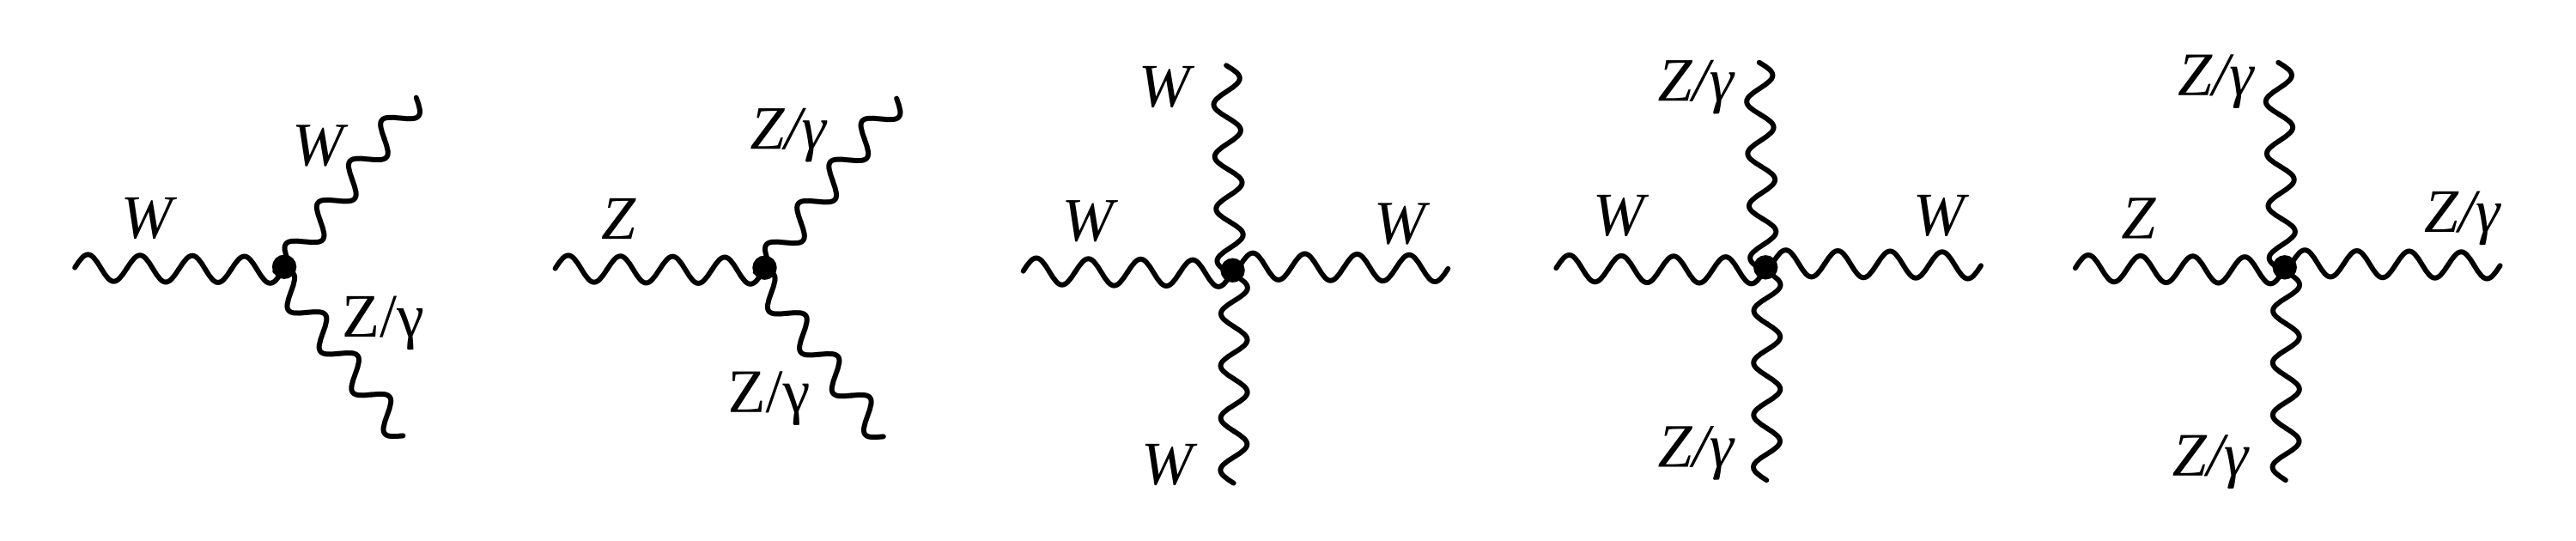
\includegraphics[width=0.95\textwidth]{../figs/WgAbout/TGC_and_QGC_vertices.png}}
    \caption{Charged TGC (first), neutral TGC (second), charged QGC (third and fourth), and neutral QGC (fifth) vertices.}
    \label{fig:TGC_and_QGC_vertices}
  \end{center}
\end{figure}

To account for the effects from the potential loops of heavy particles, we introduce an effective Lagrangian with arbitrary values of coupling constants which can be reduced to the SM Lagrangian if these constants would have their SM values. Introducing the effective Lagrangian makes searches model-independent because we do not specify particles that form the loops but instead just check whether there is a deviation from the SM prediction in measured observables. \\

In $W\gamma$ measurement we can probe $WW\gamma$ vertex. The most general Lorentz invariant Lagrangian terms of $WW\gamma$ interaction takes the following form~\cite{ref_theory_aTGC}:\\

\begin{equation}\label{L_ATGC}
i L_{eff}^{WW\gamma}= i L_{eff(1)}^{WW\gamma} + i L_{eff(2)}^{WW\gamma} + i L_{eff(3)}^{WW\gamma},
\end{equation}
\noindent{where}\\

\begin{equation}\label{L_ATGC_1}
i L_{eff(1)}^{WW\gamma}= e [ g_1^{\gamma} A^\mu (W_{\mu\nu}^- W^{+\nu} - W_{\mu\nu}^+ W^{-\nu}) + \kappa_\gamma W_{\mu}^+ W_{\nu}^- A^{\mu\nu} + {\frac{\lambda_\gamma}{m^2_W}} A^{\mu\nu} W_\nu^{+\rho} W_{\rho\mu}^- ],
\end{equation}

\begin{equation}\label{L_ATGC_2}
i L_{eff(2)}^{WW\gamma}= e [ i g_5^\gamma \epsilon_{\mu\nu\rho\sigma}((\partial^\rho W^{-\mu})W^{+\nu} - W^{-\mu}(\partial^{\rho}W^{+\nu}))A^\sigma + i g_4^\gamma W_\mu^- W_\nu^+ (\partial^\mu A^\nu + \partial^\nu A^\mu) ],
\end{equation}

\begin{equation}\label{L_ATGC_3}
i L_{eff(3)}^{WW\gamma}= e [ \frac{\tilde{\kappa_\gamma}}{2} W_\mu^- W_\nu^+ \epsilon^{\mu\nu\rho\sigma} A_{\rho\sigma} - \frac{\tilde{\lambda_\gamma}}{2 m_W^2} W_{\rho\mu}^- W^{+\mu}_{\nu} \epsilon^{\nu\rho\alpha\beta} A_{\alpha\beta}],
\end{equation}

\noindent{where $e$ is the absolute value of the electron charge, $A^\mu$ is the photon field, $W^{\pm\mu}$ are fileds of $W^\pm$ bosons, $W_{\mu\nu}=\partial_\mu W_\nu - \partial_\nu W_\mu$, $A_{\mu\nu}=\partial_\mu A_\nu - \partial_\nu A_\mu$, $m_W$ is the mass of a $W$ boson, $g_1^\gamma$, $\kappa_\gamma$, $\lambda_\gamma$, $g_5^\gamma$, $g_4^\gamma$, $\tilde{\kappa_\gamma}$, and $\tilde{\lambda_\gamma}$ are constants}.\\

Despite seven constants in the extended Lagrangian, only $\lambda_\gamma$ and $\kappa_\gamma$ are considered in the aTGC searches. The rest of the constants are fixed to their SM values based on the following considerations. The constants $g_1^\gamma=1$ and $g_5^\gamma=0$ are fixed to make the Lagrangian obey the electromagnetic gauge invariance for the on-shell photons. The non-zero value of $g_5^\gamma$ also violates C and P conservations, and non-zero values of $g_4^\gamma$, $\tilde{\kappa_\gamma}$, $\tilde{\lambda_\gamma}$ violate the CP conservation law. Such violation parametrizations are not considered in charged TGC measurements, thus, constants $g_4^\gamma$, $\tilde{\kappa_\gamma}$, and $\tilde{\lambda_\gamma}$ are fixed to zero.\\

The SM values of $\lambda_\gamma$ and $\kappa_\gamma$ are $\lambda_\gamma=0$ and $\kappa_\gamma=1$. For convenience, the deviation from the SM value is introduced $\Delta \kappa_\gamma \equiv \kappa_\gamma-1$. These two parameters are tested in $WW\gamma$ aTGC searches because non-zero values of these parameters would not violate any fundamental law.\\

The most significant effects of aTGC would appear at high energy scales. Figure~\ref{fig:aTGC_Pt_Wg} shows this effect in $P_T^\gamma$ spectrum of~7~TeV $W\gamma \rightarrow \mu\nu\gamma$ measurement. As seen in Fig.~\ref{fig:aTGC_Pt_Wg} the spectrum with non-zero values of aTGC constants at low $P_T^{\gamma}$ coincides with the SM prediction but for higher $P_T^{\gamma}$ the disagreement appears.\\

A common approach to aTGC searches is measuring a spectrum of a kinematic parameter highly correlated with an energy of a final state particle or a system of final state particles. For $W\gamma$ process, the most sensitive variable is $P_T^\gamma$. Examining this spectrum allows us to probe and constrain aTGC coupling constants. Chapter~\ref{sec:WgAbout_PastMeas} reviews the experimental results to date on constraining aTGC coupling constants of $WW\gamma$ vertex.\\ 

\begin{figure}[htb]
  \begin{center}
    {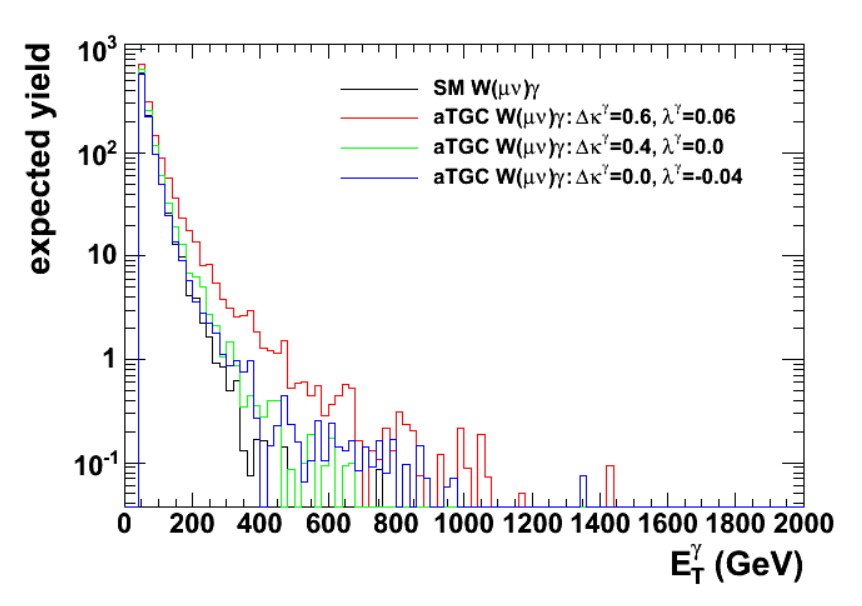
\includegraphics[width=0.85\textwidth]{../figs/WgAbout/aTGC_Pt_Wg.png}}
    \caption{Distributions of $P_T^\gamma$ of simulated $W\gamma\rightarrow\mu\nu\gamma$ events with different values of aTGC constants at LHC energy of $\sqrt{s}=7$~TeV. Source of figure:  \cite{ref_Senka_thesis}.}
    \label{fig:aTGC_Pt_Wg}
  \end{center}
\end{figure}

%\begin{figure}[htb]
%  \begin{center}
%    {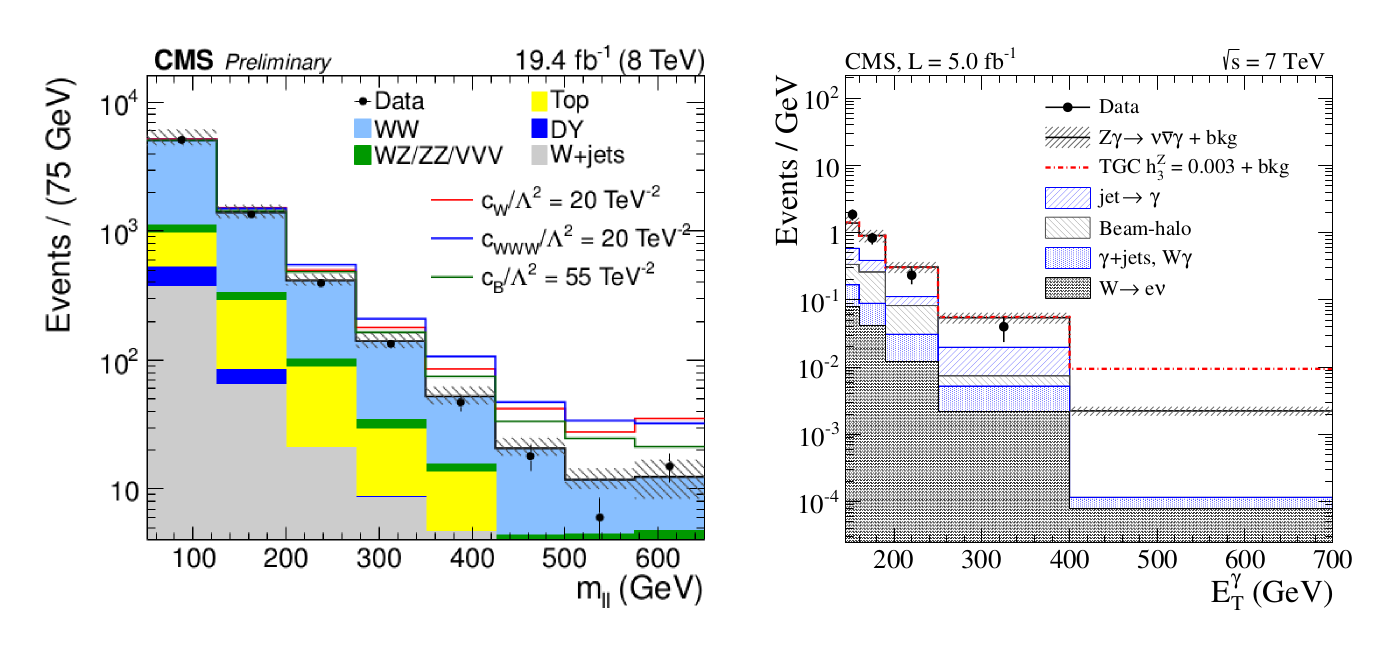
\includegraphics[width=0.85\textwidth]{../figs/WgAbout/aTGC_Pt_Examples.png}}
%    \caption{Examples of the potential effects of non-zero TGC constants in $m_{ll}$ spectrum in 8 TeV $WW \rightarrow l\nu l\nu$ measurement (left) \cite{ref_CMS_8TeV_WW} and $P_T^{\gamma}$ spectrum in 7 TeV $Z\gamma \rightarrow \nu\nu\gamma$ measurement (right) \cite{ref_CMS_7TeV_Zgnunug}.}
%    \label{fig:aTGC_Pt_Examples}
%  \end{center}
%\end{figure}
